% \documentclass[11pt,aspectratio=169]{beamer}

% \usetheme{Madrid}
% \usecolortheme{default}

% \usepackage[utf8]{inputenc}
% \usepackage[utf8]{vietnam}
% \usepackage{amsmath}
% \usepackage{amsfonts}
% \usepackage{amssymb}
% \usepackage{graphicx}
% \usepackage{booktabs}
% \usepackage{tikz}
% \usepackage{array}
% \usepackage{multirow}

% % Colors
% \definecolor{uetblue}{RGB}{0,83,159}
% \definecolor{accent}{RGB}{200,50,50}
% \definecolor{lightgray}{RGB}{245,245,245}
% \definecolor{darkgreen}{RGB}{0,128,0}

% \setbeamercolor{title}{fg=white,bg=uetblue}
% \setbeamercolor{frametitle}{fg=white,bg=uetblue}
% \setbeamercolor{structure}{fg=uetblue}
% \setbeamercolor{block title}{bg=uetblue,fg=white}

% \setbeamertemplate{caption}[numbered]
% \setbeamertemplate{navigation symbols}{}
% \setbeamertemplate{footline}{%
%   \leavevmode%
%   \hbox{%
%     \begin{beamercolorbox}[wd=.5\paperwidth,ht=2.5ex,dp=1ex,left]{author in head/foot}%
%       \hspace*{2ex}\insertshortauthor
%     \end{beamercolorbox}%
%     \begin{beamercolorbox}[wd=.5\paperwidth,ht=2.5ex,dp=1ex,right]{date in head/foot}%
%       \insertframenumber{}/\inserttotalframenumber\hspace*{2ex}
%     \end{beamercolorbox}%
%   }%
% }

% \author{Vũ Quang Sơn}
% \title{Phân loại hệ gen thực khuẩn\\dựa trên phương pháp học sâu}
% \subtitle{Luận văn Thạc sĩ Công nghệ thông tin}
% \institute{Đại học Công nghệ -- ĐHQGHN\\[0.3em]
% \small Giảng viên hướng dẫn: TS. Điệp Thị Hoàng}
% \date{05-2026}

% \begin{document}

% % ============================================================
% \begin{frame}
% \titlepage
% \end{frame}

% % ============================================================
% \begin{frame}{Nội dung trình bày}
% \tableofcontents
% \end{frame}

% % ============================================================
% \section{Động lực nghiên cứu}
% \begin{frame}{Động lực nghiên cứu}

% \begin{columns}[T]
% \begin{column}{0.45\textwidth}
% \vspace{1em}

% \textbf{\large Thực khuẩn thể (phage)}

% \vspace{0.5em}
% \begin{itemize}\setlength{\itemsep}{6pt}
%     \item \textcolor{accent}{\textbf{Độc lực}} $\rightarrow$ chu trình tan, tấn công vào gen vật chủ
%     \item \textcolor{uetblue}{\textbf{Ôn hòa}} $\rightarrow$ có chu trình tiềm tan, tích hợp vào gen vật chủ
% \end{itemize}

% \vspace{1em}
% \textbf{\large Tại sao cần phân loại?}

% \vspace{0.5em}
% \begin{itemize}\setlength{\itemsep}{6pt}
%     \item Liệu pháp phage: \textbf{chỉ dùng độc lực}
%     \item Ôn hòa $\rightarrow$ truyền gen kháng kháng sinh
% \end{itemize}
% \end{column}

% \begin{column}{0.50\textwidth}
% \vspace{1em}

% \textbf{\large Động lực nghiên cứu}

% \begin{itemize}
%     \item Các phương pháp nuôi cấy truyền thống tốn nhiều chi phí và thời gian.
% \end{itemize}

% \end{column}
% \end{columns}

% \end{frame}

% % ============================================================
% \section{Phát biểu bài toán}
% \begin{frame}{Phát biểu bài toán}

% \begin{center}
% \begin{tikzpicture}[
%     box/.style={draw=uetblue, rounded corners, fill=lightgray,
%                 minimum height=1.1cm, align=center, font=\small},
%     arrow/.style={->, thick, uetblue}
% ]

% % Input
% \node[box, text width=3.5cm] (input) at (0,0) {
%     \textbf{Đầu vào}\\[2pt]
%     $s \in \{A,T,G,C\}^L$\\
%     $L \in [100,\; 1800]$ bp
% };

% % Model
% \node[box, text width=3.2cm] (model) at (5,0) {
%     \textbf{Mô hình}\\[2pt]
%     $f_{\theta_g}: \mathcal{S}_g \rightarrow \{0,1\}$
% };

% % Output
% \node[box, text width=3.2cm] (output) at (9.8,0) {
%     \textbf{Đầu ra}\\[2pt]
%     $y=0$: Ôn hòa\\
%     $y=1$: Độc lực
% };

% % Arrows
% \draw[arrow] (input) -- (model);
% \draw[arrow] (model) -- (output);



% % Length groups below
% \node[draw=uetblue!60, rounded corners, fill=uetblue!8,
%       text width=11cm, align=center, font=\small] at (4.9,-2.2) {
%     % \textbf{4 nhóm:}\;
%     % A: 100--400\;|\;
%     % B: 400--800\;|\;
%     % C: 800--1200\;|\;
%     % D: 1200--1800 (bp)\\[3pt]
%     % Mỗi nhóm $g$ có mô hình $f_{\theta_g}$ riêng biệt
%     \begin{itemize}
%         \item Dữ liệu đầu vào được chia thành 4 nhóm: A (100--400), B(400--800), C(800--1200), D(1200--1800)
%         \item Mỗi nhóm được thực hiện xử lý trên 1 mô hình riêng
%     \end{itemize}
% };

% \end{tikzpicture}
% \end{center}

% \end{frame}

% % ============================================================
% \section{Hạn chế phương pháp hiện có}
% \begin{frame}{Nghiên cứu liên quan}

% \vspace{0.3em}
% \begin{table}
% \centering
% \small
% \begin{tabular}{l l l}
% \toprule
% \textbf{Phương pháp} & \textbf{Biểu diễn} & \textbf{Hạn chế chính} \\
% \midrule
% PhaTYP & Protein (BERT) & Cần Prodigal phát hiện protein $\rightarrow$ fail contig ngắn \\
% DeePhage & One-hot (CNN) & Không tận dụng các mô hình tiền huấn luyện \\
% ProkBERT & LCA k-mer (BERT) & Sử dụng K-mer chồng lần $\rightarrow$ Rò rỉ thông tin \\
% DeepPL & k-mer (DNABERT) & Giới hạn độ dài dữ liệu đầu vào 512bp cho 1 cửa sổ \\
% \bottomrule
% \end{tabular}
% \end{table}

% \vspace{0.8em}
% \begin{center}
% \begin{tikzpicture}
% \node[draw=accent, rounded corners, fill=accent!8,
%       text width=10cm, align=center, font=\normalsize] {
%     Cần một phương pháp có thể khắc phục các nhược điểm trên
% };
% \end{tikzpicture}
% \end{center}

% \end{frame}

% % ============================================================
% \section{Phương pháp đề xuất}
% \begin{frame}{Kiến trúc PhaBERT}

% \vspace{0.5em}
% \textbf{Kiến trúc PhaBERT:} là sự kết hợp của mô hình nền tảng DNABERT-2 và mô-đun MKC(Multi-Kernal Convolutional) gồm nhiều nhánh CNN có kích thước độ cửa sổ tích chập khác nhau cùng 1 nhánh pooling toàn cục với các ưu điểm:
% \begin{enumerate}\setlength{\itemsep}{12pt}
%     \item[\textcolor{uetblue}{\textbf{1}}] Xử lý trực tiếp trên chuỗi DNA thô, độ dài bất kỳ, không cần công cụ tiền xử lý.\\[3pt]
%     \item[\textcolor{uetblue}{\textbf{2}}] Sử dụng BPE trong quá trình tokenization nên không rỏ rỉ thông tin.\\[3pt]
%     \item[\textcolor{uetblue}{\textbf{3}}] Kết hợp mô hình xử lý chuyên biệt với mô hình nền tảng cho hiệu suất tối ưu trên bài toán.\\[3pt]
% \end{enumerate}

% \end{frame}

% % ============================================================
% % \section{Mô hình đề xuất}
% \begin{frame}[plain]{Kiến trúc PhaBERT}

% \begin{columns}[T]
% \begin{column}{0.30\textwidth}
% \vspace{1.5em}

% \textbf{2 thành phần:}
% \begin{enumerate}\setlength{\itemsep}{8pt}
%     \item DNABERT-2
%     \item MKC
%     \begin{itemize}
%         \item Các nhánh CNN
%         \item Nhánh pooling
%         \item Đầu phân loại
%     \end{itemize}
% \end{enumerate}
% \end{column}

% \begin{column}{0.68\textwidth}
% \centering
% 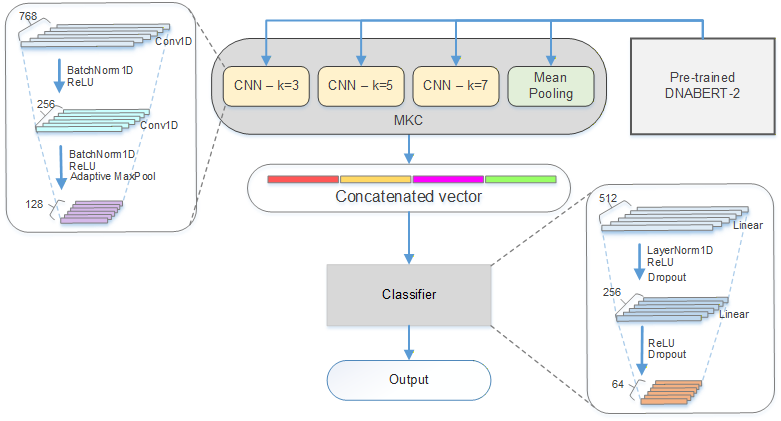
\includegraphics[width=\textwidth,height=0.85\textheight,keepaspectratio]{figures/phabert-cnn.png}
% \end{column}
% \end{columns}

% \end{frame}

% % ============================================================
% % \section{Dữ liệu \& Tiền xử lý}
% \begin{frame}{Dữ liệu và tiền xử lý}

% \begin{columns}[T]
% \begin{column}{0.35\textwidth}
% \vspace{0.5em}

% \textbf{2.241} hệ gen phage\\[4pt]
% 707 ôn hòa + 1.534 độc lực\\[4pt]
% 5-fold cross-validation

% \vspace{1em}
% \textbf{3 bước xử lý:}
% \begin{enumerate}\setlength{\itemsep}{4pt}
%     \item Cửa sổ trượt tạo contig
%     \item Tăng cường dữ liệu với đảo ngược bổ sung
%     \item Cân bằng tỷ lệ nhãn với Random Undersampling
% \end{enumerate}
% \end{column}

% \begin{column}{0.63\textwidth}
% \centering
% 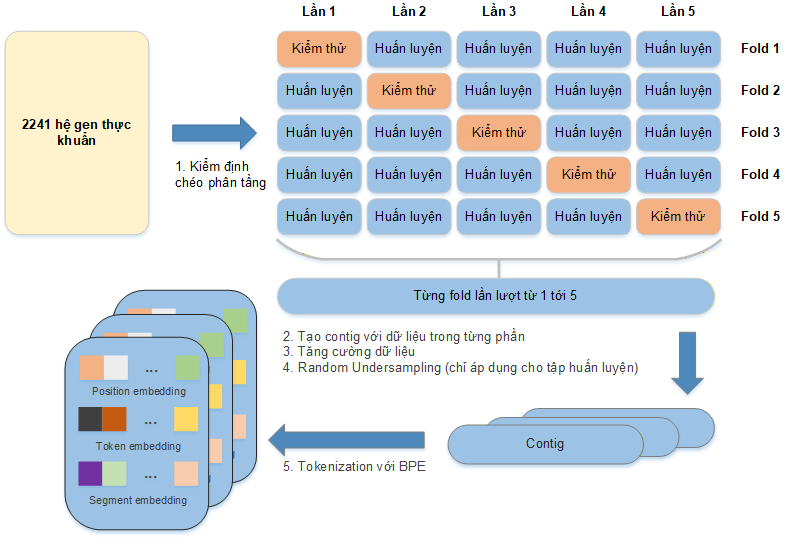
\includegraphics[width=\textwidth,height=0.78\textheight,keepaspectratio]{figures/data_preparation.png}
% \end{column}
% \end{columns}

% \end{frame}

% % ============================================================
% % \begin{frame}{Chiến lược huấn luyện}

% \begin{columns}[T]
% \begin{column}{0.45\textwidth}
% \vspace{0.5em}

% \begin{tikzpicture}[
%     phase/.style={draw=uetblue, rounded corners, fill=uetblue!8,
%                   text width=5cm, minimum height=1.5cm, align=left, font=\small},
%     arrow/.style={->, thick, uetblue}
% ]
% \node[phase] (p1) at (0,0) {
%     \textbf{GĐ1: Freeze backbone}\\[2pt]
%     Đóng băng DNABERT-2\\
%     Chỉ huấn luyện mô-đun MKC\\
%     1 epochs
% };
% \node[phase] (p2) at (0,-3) {
%     \textbf{GĐ2: Unfreeze all}\\[2pt]
%     Tinh chỉnh toàn bộ mô hình\\
%     Mỗi phần có tốc độ học phân biệt\\
%     10 epochs
% };
% \draw[arrow] (p1) -- (p2);
% \end{tikzpicture}
% \end{column}
% \end{columns}

% \end{frame}

% % ============================================================
% \section{Kết quả thực nghiệm}
% \begin{frame}{Thiết lập thực nghiệm}

% \vspace{0.3em}
% \textbf{Phương pháp đánh giá:}
% \begin{itemize}\setlength{\itemsep}{4pt}
%     \item Kiểm định chéo phân tầng 5 phần
%     \item Tỷ lệ train:val = 8:2
%     \item Undersampling chỉ trên tập train
% \end{itemize}

% \vspace{0.8em}
% \textbf{Chỉ số:}
% \begin{itemize}\setlength{\itemsep}{4pt}
%     \item Sn (Sensitivity): nhận diện thực khuận có độc lực
%     \item Sp (Specificity): nhận diện thực khuẩn ôn hòa
%     \item Acc (Accuracy): tổng thể
% \end{itemize}

% \end{frame}

% % ============================================================
% \begin{frame}{Kết quả so sánh}

% \vspace{-0.2em}
% \begin{table}
% \centering
% \begin{tabular}{l c c c c}
% \toprule
% \textbf{Phương pháp} & \textbf{A} & \textbf{B} & \textbf{C} & \textbf{D} \\
%  & {\scriptsize 100-400bp} & {\scriptsize 400-800bp} & {\scriptsize 800-1200bp} & {\scriptsize 1200-1800bp} \\
% \midrule
% \textbf{PhaBERT}     & \textbf{82,01} & \textbf{87,33} & \textbf{89,90} & \textbf{91,38} \\
% PhaTYP               & 78,92 & 85,90 & 88,87 & 91,02 \\
% DeePhage             & 78,07 & 84,17 & 87,37 & 89,09 \\
% ProkBERT             & 80,68 & 85,35 & 84,03 & 84,73 \\
% DNABERT-2            & 81,52 & 85,56 & 87,25 & 88,36 \\
% \bottomrule
% \multicolumn{5}{r}{\scriptsize Chỉ số: Accuracy (\%) -- 5-fold stratified cross-validation}
% \end{tabular}
% \end{table}

% \vspace{0.3em}
% {\small
% \begin{itemize}\setlength{\itemsep}{2pt}
%     \item PhaBERT cho chỉ số accuracy cao nhất so với các phương pháp còn lại
%     % \item Hiệu suất tăng dần theo độ dài contig (82\% $\rightarrow$ 91\%)
%     % \item ProkBERT bão hòa từ nhóm B $\rightarrow$ hạn chế k-mer chồng lấn
% \end{itemize}
% }

% \end{frame}

% % ============================================================
% \begin{frame}{Phân tích Sensitivity/Specificity}

% \begin{columns}[T]
% \begin{column}{0.55\textwidth}
% \centering
% 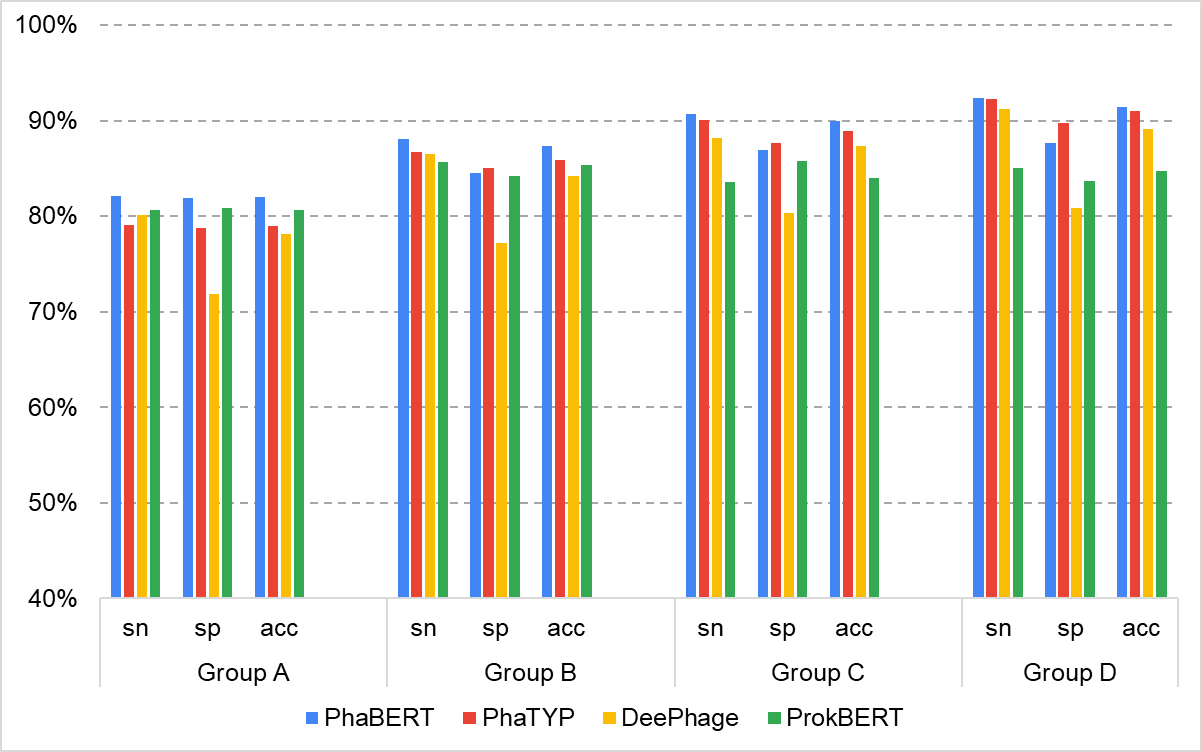
\includegraphics[width=\textwidth,height=0.78\textheight,keepaspectratio]{figures/exp_2.png}
% \end{column}

% \begin{column}{0.43\textwidth}
% \vspace{1em}

% \vspace{0.5em}
% {\small
% \begin{itemize}\setlength{\itemsep}{6pt}
%     \item PhaBERT cho Sn cao nhất mọi nhóm (82--92\%)\\
%     $\rightarrow$ phát hiện tốt phage độc lực

%     \item PhaTYP Sp tốt hơn ở 3 nhóm (B, C, D)
%     $\rightarrow$ nhờ đặc trưng cấp độ protein
% \end{itemize}
% }
% \end{column}
% \end{columns}

% \end{frame}

% % ============================================================
% \begin{frame}{Ablation Study}

% \centering
% 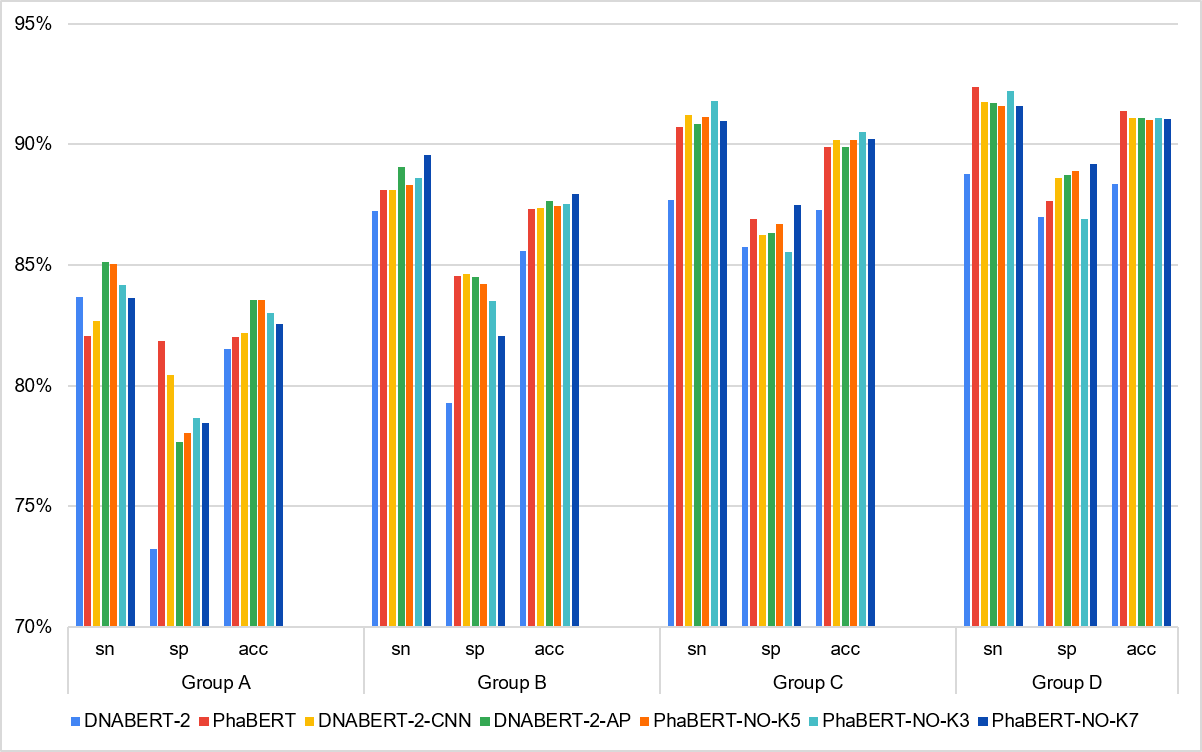
\includegraphics[width=\textwidth,height=0.78\textheight,keepaspectratio]{figures/ablation_test.png}

% \end{frame}

% % ============================================================
% \section{Hạn chế}
% \begin{frame}{Hạn chế và hướng phát triển}

% \textbf{Hạn chế}
% \begin{itemize}
%     \item Việc sử dụng Random Undersampling có thể mất thông tin quan trọng 
%     \item Mô hình hiện tại chỉ sử dụng đặc trưng cấp độ nucleotide.
% \end{itemize}

% \textbf{Hướng phát triển}
% \begin{itemize}
%     \item Sử dụng phương pháp xử lý mất cân bằng nhãn khác để không làm mất dữ liệu
%     \item Kết hợp đặc trưng cấp độ protein.
% \end{itemize}

% \end{frame}

% % ============================================================
% \begin{frame}{}
% \begin{center}
% \vspace{2em}
% {\Huge\color{uetblue} Cảm ơn thầy cô!}

% \vspace{1.5em}
% \textbf{Vũ Quang Sơn}\\
% Trường Đại học Công nghệ -- ĐHQGHN
% \end{center}
% \end{frame}

% % ============================================================
% % BACKUP SLIDES
% % ============================================================

% \appendix
% \newcounter{backupslide}
% \setcounter{backupslide}{0}

% % ============================================================
% \begin{frame}{Thống kê dữ liệu chi tiết}

% \vspace{0.3em}
% {\small
% \begin{table}
% \centering
% \begin{tabular}{l l r r r}
% \toprule
% \textbf{Nhóm} & \textbf{Tập} & \textbf{Ôn hòa} & \textbf{Độc lực} & \textbf{Tổng} \\
% \midrule
% \multirow{2}{*}{A (100--400 bp)} & Huấn luyện & 230.156 & 230.156 & 460.312 \\
%  & Kiểm định & 57.366 & 215.054 & 272.420 \\
% \midrule
% \multirow{2}{*}{B (400--800 bp)} & Huấn luyện & 95.750 & 95.750 & 191.500 \\
%  & Kiểm định & 23.804 & 89.404 & 113.208 \\
% \midrule
% \multirow{2}{*}{C (800--1200 bp)} & Huấn luyện & 55.024 & 55.024 & 110.048 \\
%  & Kiểm định & 13.694 & 51.424 & 65.118 \\
% \midrule
% \multirow{2}{*}{D (1200--1800 bp)} & Huấn luyện & 42.780 & 42.780 & 85.560 \\
%  & Kiểm định & 10.640 & 39.960 & 50.600 \\
% \bottomrule
% \end{tabular}
% \end{table}
% }

% \vspace{0.3em}
% {\small Số liệu sau tăng cường (RC). Undersampling 1:1 chỉ áp dụng trên tập huấn luyện.}

% \end{frame}

% \begin{frame}{Ablation đầy đủ 7 cấu hình}

% \vspace{-0.3em}
% \resizebox{\textwidth}{!}{%
% \scriptsize
% \begin{tabular}{l c c c c c c c c c c c c}
% \toprule
% & \multicolumn{3}{c}{\textbf{Nhóm A}} & \multicolumn{3}{c}{\textbf{Nhóm B}} & \multicolumn{3}{c}{\textbf{Nhóm C}} & \multicolumn{3}{c}{\textbf{Nhóm D}} \\
% \cmidrule(lr){2-4}\cmidrule(lr){5-7}\cmidrule(lr){8-10}\cmidrule(lr){11-13}
% \textbf{Cấu hình} & Sn & Sp & Acc & Sn & Sp & Acc & Sn & Sp & Acc & Sn & Sp & Acc \\
% \midrule
% DNABERT-2 & 83,68 & 73,25 & 81,52 & 87,24 & 79,27 & 85,56 & 87,68 & 85,75 & 87,25 & 88,75 & 86,99 & 88,36 \\
% \textbf{PhaBERT} & 82,07 & \textbf{81,86} & 82,01 & 88,11 & 84,53 & 87,33 & 90,69 & \textbf{86,92} & 89,90 & \textbf{92,38} & 87,63 & \textbf{91,38} \\
% DNABERT-2-CNN & 82,68 & 80,44 & 82,18 & 88,11 & \textbf{84,63} & 87,36 & \textbf{91,21} & 86,25 & \textbf{90,16} & 91,75 & 88,58 & 91,07 \\
% DNABERT-2-P & \textbf{85,12} & 77,65 & \textbf{83,54} & \textbf{89,04} & 84,49 & \textbf{87,63} & 90,84 & 86,30 & 89,88 & 91,72 & \textbf{88,74} & 91,08 \\
% PhaBERT-NO-K5 & 85,05 & 78,03 & 83,56 & 88,31 & 84,19 & 87,44 & 91,12 & 86,71 & 90,18 & 92,22 & 86,92 & 90,99 \\
% PhaBERT-NO-K3 & 84,18 & 78,65 & 83,00 & 88,61 & 83,50 & 85,51 & 91,80 & 85,53 & 90,49 & 92,22 & 86,92 & 91,05 \\
% PhaBERT-NO-K7 & 83,62 & 78,47 & 82,55 & 89,54 & 82,06 & 87,95 & 90,95 & 87,47 & 90,21 & 91,56 & 89,20 & 91,05 \\
% \bottomrule
% \end{tabular}%
% }

% \end{frame}

% % ============================================================
% \begin{frame}{So sánh chi tiết với các phương pháp tiên tiến}

% \vspace{-0.3em}
% \resizebox{\textwidth}{!}{%
% \scriptsize
% \begin{tabular}{l c c c c c c c c c c c c}
% \toprule
% & \multicolumn{3}{c}{\textbf{Nhóm A (100--400 bp)}} & \multicolumn{3}{c}{\textbf{Nhóm B (400--800 bp)}} & \multicolumn{3}{c}{\textbf{Nhóm C (800--1200 bp)}} & \multicolumn{3}{c}{\textbf{Nhóm D (1200--1800 bp)}} \\
% \cmidrule(lr){2-4}\cmidrule(lr){5-7}\cmidrule(lr){8-10}\cmidrule(lr){11-13}
% \textbf{Phương pháp} & Sn & Sp & Acc & Sn & Sp & Acc & Sn & Sp & Acc & Sn & Sp & Acc \\
% \midrule
% \textbf{PhaBERT} & \textbf{82,07} & \textbf{81,86} & \textbf{82,01} & \textbf{88,11} & 84,53 & \textbf{87,33} & \textbf{90,69} & 86,92 & \textbf{89,90} & \textbf{92,38} & 87,63 & \textbf{91,38} \\
% PhaTYP & 79,07 & 78,77 & 78,92 & 86,74 & \textbf{85,06} & 85,90 & 90,09 & \textbf{87,65} & 88,87 & 92,29 & \textbf{89,75} & 91,02 \\
% DeePhage & 80,09 & 71,79 & 78,07 & 86,46 & 77,18 & 84,17 & 88,20 & 80,31 & 87,37 & 91,17 & 80,84 & 89,09 \\
% ProkBERT & 80,65 & 80,80 & 80,68 & 85,67 & 84,15 & 85,35 & 83,61 & 85,72 & 84,03 & 85,00 & 83,68 & 84,73 \\
% \bottomrule
% \end{tabular}%
% }

% \vspace{0.5em}
% {\small Kiểm định chéo phân tầng 5 phần. Sn = Độ nhạy, Sp = Độ đặc hiệu, Acc = Độ chính xác.}

% \end{frame}

% % ============================================================
% \begin{frame}{Thuật toán Byte Pair Encoding (BPE)}

% \begin{columns}[T]
% \begin{column}{0.45\textwidth}
% \vspace{0.3em}

% \textbf{Thuật toán:}
% \begin{enumerate}\setlength{\itemsep}{6pt}
%     \item Khởi tạo từ điển $V = \{A, T, G, C\}$
%     \item Đếm tần suất mọi cặp token liền kề
%     \item Ghép cặp có tần suất cao nhất $\rightarrow$ token mới
%     \item Lặp bước 2--3 cho đến $|V| = 4.096$
% \end{enumerate}

% \vspace{0.8em}
% \textbf{Kết quả:}
% \begin{itemize}\setlength{\itemsep}{4pt}
%     \item Token có độ dài biến đổi, trung bình $\approx$ 5 nt/token
%     \item Giảm $\sim$5$\times$ độ dài chuỗi so với k-mer
%     \item Không chồng lấn $\rightarrow$ loại bỏ rò rỉ thông tin
% \end{itemize}
% \end{column}

% \begin{column}{0.52\textwidth}
% \vspace{0.3em}

% \textbf{Ví dụ trên chuỗi DNA:}

% \vspace{0.5em}
% {\ttfamily\small
% \begin{tabular}{@{}l l@{}}
% Gốc: & A T C G A T C G A T G C \\[6pt]
% Bước 1: & \fbox{AT} C G \fbox{AT} C G \fbox{AT} G C \\
%         & {\scriptsize (ghép ``AT'' -- tần suất cao nhất)} \\[6pt]
% Bước 2: & AT \fbox{CG} AT \fbox{CG} AT G C \\
%         & {\scriptsize (ghép ``CG'')} \\[6pt]
% Bước 3: & \fbox{ATCG} \fbox{ATCG} AT G C \\
%         & {\scriptsize (ghép ``AT''+``CG'')} \\
% \end{tabular}
% }

% \vspace{0.8em}
% \begin{center}
% \begin{tikzpicture}
% \node[draw=accent, rounded corners, fill=accent!8,
%       text width=5cm, align=center, font=\small] {
%     Mỗi nucleotide thuộc\\đúng 1 token duy nhất
% };
% \end{tikzpicture}
% \end{center}
% \end{column}
% \end{columns}

% \end{frame}

% \end{document}
